\section{Задание 1}

Оформить задание 2 из Лабораторной работы 1 в виде функции и вызвать эту функцию по нажатию кнопки.

\begin{center}
  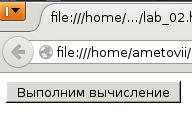
\includegraphics{img/01.png}

  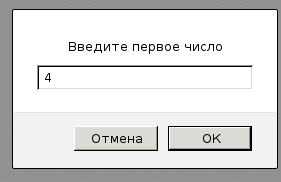
\includegraphics{img/02.png}
  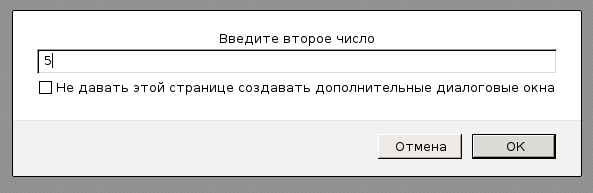
\includegraphics{img/03.png}
  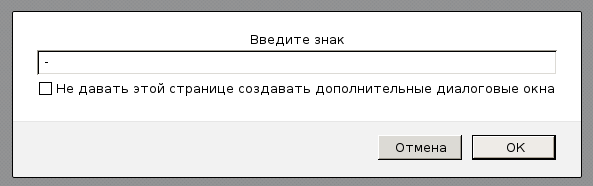
\includegraphics{img/04.png}
  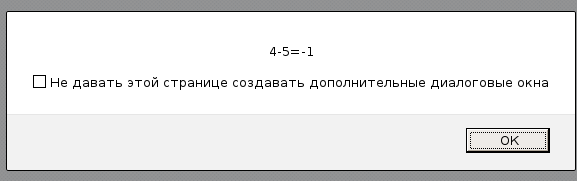
\includegraphics{img/05.png}
\end{center}

Остальные операции аналогичны. Исходный код \verb|lab_02.html|:

\begin{verbatim}
<html>
  <head>
    <meta charset="utf-8">
    <script>
      function chet()
      {
          a = parseInt (prompt ("Введите первое число"))
          b = parseInt (prompt ("Введите второе число"))
          operation = prompt ("Введите знак")
          switch (operation) {
          case "*":
              alert (a + operation + b + "="
                     + (a * b))
              break
          case "+":
              alert (a + operation + b + "="
                     + (a + b))
              break
          case "-":
              alert (a + operation + b + "="
                     + (a - b))
              break
          case "/":
	      if (b==0) {alert ("Ошибка! На ноль " +
				"делить нельзя")}
              else {alert (a + operation + b + "="
                           + (a / b))}
              break
          default:
	      alert ("Ошибка! Недопустимый "+
		     "знак операции!")
              break
          }
      }
    </script>
  </head>
  <body>
    <input type="button" value="Выполним вычисление"
	   onClick="chet()">
  </body>
</html>
\end{verbatim}
